\section{Geometrieaufgaben durchrechnen}\label{kapitel:Durchrechnen}
Wenn ihr bei einer Geometrieaufgabe stecken bleibt, drängt sich früher oder später unweigerlich der Gedanke auf, ob sich die Aufgabe nicht einfach durchrechnen ließe. In diesem Abschnitt wollen wir besprechen, wie ihr damit erfolgreich sein könnt und was ihr vermeiden solltet.

\textbf{Einige Warnungen vorweg.}
Ihr solltet euch folgender Dinge bewusst sein:
\begin{itemize}[label=\Warnung]
	\item Durchrechnen ist nicht gern gesehen. Unvollständige Durchrechenlösungen werden in der Regel sehr hart bewertet. Bei der IMO ist es sogar so streng, dass unvollständige Durchrechenlösungen überhaupt keine Punkte bekommen. Lediglich Zwischenergebnisse, die zurück in die Sprache der Geometrie übersetzt wurden, werden honoriert.
	\item Durchrechnen ist fehleranfällig. Die Korrekturerfahrung zeigt, dass die meisten Durchrechenversuche an Umformungsfehlern scheitern. Je nachdem, wie früh ein solcher Fehler passiert, kann er sich auf fatale Weise fortpflanzen und seitenlange Rechnungen wertlos machen. Selbst bei weniger strengen Wettbewerben als der IMO werden solche Abgaben in der Regel mit sehr bescheidenen Punktzahlen bedacht.
	\item Durchrechnen ist zeitaufwendig, besonders dann, wenn ihr merkt, dass ihr euch verrechnet habt, und ihr den Fehler suchen müsst.
\end{itemize}

Deswegen solltet ihr die folgenden Ratschläge beachten:
\begin{itemize}
	\item Fangt nur an, eine Aufgabe durchzurechnen, wenn ihr euch einigermaßen sicher seid, dass ihr durchkommt.
	\item Macht euch vorher einen Plan: Welche Punkte sind am schwierigsten zu berechnen? Welche Annahmen und Vereinfachungen könnt ihr treffen, um die schwierigsten Schritte so einfach wie möglich zu machen?
	\item Versucht die Aufgabe immer zuerst elementar zu lösen. Denn selbst, wenn ihr euch später entschließt, die Aufgabe durchzurechnen, gibt es häufig einfache elementare Beobachtungen, die euch das Durchrechnen wesentlich erleichtern. Und wenn ihr beim Durchrechnen doch nicht erfolgreich seid, kriegt ihr für die elementaren Beobachtungen immerhin noch ein paar Punkte.
\end{itemize}

In meiner Erfahrung gibt es drei sinnvolle Methoden, Aufgaben durchzurechnen: Trigonometrie, komplexe Zahlen und baryzentrische Koordinaten. Cartesische Koordinaten,
% Tien: Der Duden empfiehlt "kartesische Koordinaten".
wie in der Schule, solltet ihr nur im absoluten Notfall verwenden, denn fast immer ist eine der anderen Methoden besser geeignet. Wir werden nun (kurz) das Durchrechnen mit Trigonometrie und mit komplexen Zahlen besprechen. Für baryzentrische Koordinaten gibt es zum Beispiel das sehr umfangreiche Skript \emph{Barycentric Coordinates in Olympiad Geometry} von Max Schindler und Evan Chen\footnote{Online verfügbar unter \url{https://web.evanchen.cc/handouts/bary/bary-full.pdf}}. Und zu komplexen Zahlen gibt es natürlich das berühmte Skript von Eric Müller.\footnote{Dem Autoren ist leider nicht bekannt, ob dieses online verfügbar ist.}

\subsection*{Durchrechnen mit Trigonometrie}
Die Idee hierbei ist simpel: Ihr führt einige Winkel und Streckenlängen ein und rechnet dann alle weiteren Winkel durch Winkeljagd sowie alle weiteren Längen durch den Sinus- und den Cosinussatz aus (auch die Sätze von Ceva und Menelaos sind häufig mit von der Partie; allgemein sind solche Lösungen häufig ein Mix aus elementaren Argumenten und trigonometrischen Rechnungen). Trigonometrisches Durchrechnen hat den Vorteil, dass unvollständige Lösungen weniger hart bewertet werden, weil trigonometrische Längenbeziehungen eher für nützlich erachtet werden als korrekt ausgerechnete Koordinaten.

Beim trigonometrischen Durchrechnen gilt folgende Faustregel: \emph{Der Sinussatz ist euer Freund, der Cosinussatz ist euer Feind.} Denn durch den Sinussatz bekommt ihr nur einige Faktoren hinzu, während der Cosinussatz mit Summen und Wurzeln daherkommt, die euch beim Ausmultiplizieren Kopfschmerzen bereiten werden. Natürlich lässt es sich oftmals nicht vermeiden, auch den Cosinussatz zu verwenden, aber ihr seid besser beraten, wenn ihr das Durchrechnen so strukturiert, dass der Cosinussatz möglichst wenig bzw.\ nur im letzten Schritt verwendet wird.

Ihr solltet es vermeiden, unbekannte Winkel durch $\arcsin$ oder $\arccos$ auszudrücken (es sei denn, ihr wollt zeigen, dass es sich etwa um einen $30^\circ$-~oder $60^\circ$-Winkel handelt). Versucht lieber, direkt mit Sinus oder Cosinus des betreffenden Winkels zu arbeiten.

Um trigonometrisch erfolgreich zu sein, solltet ihr selbstverständlich die Additionstheoreme im Schlaf beherrschen.
% Tien: Willst du die Additionstheoreme nochmal nennen?
Ferner solltet ihr folgende Formeln kennen (oder zumindest wissen, dass sie existieren, und sie euch herleiten können):
\begin{satzmitnamen}[Summe-zu-Produkt-Formeln]
	Für beliebige Winkel $\alpha$~und~$\beta$ gilt
	\begin{alignat*}{4}
		\sin\alpha&+\sin\beta &&= 2\sin\parens*{\tfrac{\alpha+\beta}{2}}\cos\parens*{\tfrac{\alpha-\beta}{2}}\,, & \sin\alpha&-\sin\beta &&= 2\cos\parens*{\tfrac{\alpha+\beta}{2}}\sin\parens*{\tfrac{\alpha-\beta}{2}}\,,\\
		% Tien: Habe hier ein \phantom hinzugefügt
		\cos\alpha&+\cos\beta &&= 2\cos\parens*{\tfrac{\alpha+\beta}{2}}\cos\parens*{\tfrac{\alpha-\beta}{2}}\,,\quad & \cos\alpha&-\cos\beta &&= -2\sin\parens*{\tfrac{\alpha+\beta}{2}}\sin\parens*{\tfrac{\alpha-\beta}{2}}\,.
	\end{alignat*}
\end{satzmitnamen}

Trigonometrische Lösungen enden häufig damit, dass ihr eine trigonometrische Identität nachweisen müsst. Dafür ist es neben den obigen Formeln sehr nützlich, einige Beziehungen im Dreieck zu kennen. Im Folgenden bezeichnen $a$,~$b$,~$c$ sowie $\alpha$,~$\beta$,~$\gamma$ stets die Seitenlängen und Winkelgrößen eines Dreiecks $ABC$. Wir beginnen mit einer erweiterten Form des Sinussatzes, die euch die Schule wahrscheinlich (leider) nicht so beigebracht hat.

\begin{satzmitnamen}[Erweiterter Sinussatz]
	Wenn $R$ der Umkreisradius von $ABC$ ist, dann gilt
	\begin{equation*}
		\frac{a}{\sin\alpha}=\frac{b}{\sin\beta}=\frac{c}{\sin\gamma}=2R\,.
	\end{equation*}
\end{satzmitnamen}

\begin{aufgabe*}
	Beweise die Summe-zu-Produkt-Formeln und den erweiterten Sinussatz!
\end{aufgabe*}

Als nächstes haben wir die folgenden Formeln, die dem Autoren dieses Textes in seiner eigenen Olympiadezeit gute Dienste geleistet hat:
\begin{satzmitnamen}[Halbwinkelformel]
	Sei $s\coloneqq \frac12(a+b+c)$ der halbe Umfang von $ABC$. Dann gilt
	% Tien: Dumme Frage: Muss "gilt" nicht in den Plural?
	\begin{equation*}
		\sin\parens*{\frac{\alpha}{2}}=\sqrt{\frac{(s-b)(s-c)}{bc}}\quad\text{und}\quad\cos\parens*{\frac{\alpha}{2}}=\sqrt{\frac{s(s-a)}{bc}}\,.
	\end{equation*}
\end{satzmitnamen}

\begin{proof}
	Nach Cosinussatz ist $\cos\alpha=(b^2+c^2-a^2)/(2bc)$. Damit folgen beide Behauptungen nach kurzem Umformen aus den für $0\leqslant \alpha\leqslant 180^\circ$ gültigen Halbwinkelformeln
	\begin{equation*}
		\sin\parens*{\frac{\alpha}{2}}=\sqrt{\frac{1-\cos\alpha}{2}}\quad\text{und}\quad\cos\parens*{\frac{\alpha}{2}}=\sqrt{\frac{1+\cos\alpha}{2}}\,.\qedhere
	\end{equation*}
\end{proof}
Die Halbwinkelformel ist nicht zuletzt deshalb nützlich, weil die Ausdrücke $s$ und $s-a$ auf natürliche Weise im Dreieck $ABC$ auftauchen.
\begin{aufgabe*}\label{aufgabe:s-a}
	Beweise, dass die Ausdrücke $s$ und $s-c$ als Tangentenabschnitte am In-~und Ankreis auftreten, wie sie in der untenstehenden Skizze illustriert sind. Überlege dir auch die analogen Aussagen für $s-a$ und $s-b$.
	
	\begin{figure}[ht]
		\centering
		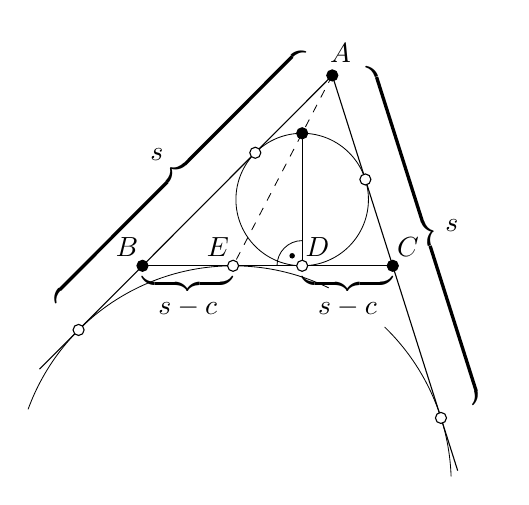
\begin{tikzpicture}[x=1.5cm,y=1.5cm]
			\draw [line width=0.3] (0.06,0.561) circle (0.561);
			\draw [line width=0.3, shift={(-0.525,-1.847)}] (64:1.847) arc (64:160:1.847);
			\draw [line width=0.3, shift={(-0.525,-1.847)}] (2:1.847) arc (2:46:1.847);
			\coordinate (A) at (0.315,1.612);
			\coordinate (B) at (-1.292,0);
			\coordinate (C) at (0.827,0);
			\coordinate (D) at (0.06,0);
			\coordinate (E) at (-0.525,0);
			\coordinate (Sb) at (0.595,0.731);
			\coordinate (Sc) at (-0.337,0.957);
			\coordinate (Tb) at (1.235,-1.288);
			\coordinate (Tc) at (-1.833,-0.543);
			\coordinate (N) at (0.06,1.122);
			\draw[shorten >=-2em] (A) to (Tc);
			\draw[shorten >=-2em] (A) to (Tb);
			\draw (B) to (C);
			\draw[dashed, line width=0.3] (A) to (E);
			\draw (D) to (N);
			\draw [line width=0.3,shift={(D)}] (90:0.32cm) arc (90:180:0.32cm);
			\fill [shift={(D)}] (135:0.18cm) circle (1pt);
			\draw[fill=black] (A) circle (2pt) node[shift={(70:2ex)}] {$A$};
			\draw[fill=black] (B) circle (2pt) node[shift={(130:2ex)}] {$B$};
			\draw[fill=black] (C) circle (2pt) node[shift={(50:2ex)}] {$C$};
			\draw[fill=white] (D) circle (2pt) node[shift={(50:2ex)}] {$D$};
			\draw[fill=white] (E) circle (2pt) node[shift={(130:2ex)}] {$E$};
			\draw[fill=white] (Sb) circle (2pt);
			\draw[fill=white] (Sc) circle (2pt);
			\draw[fill=white] (Tb) circle (2pt);
			\draw[fill=white] (Tc) circle (2pt);
			\draw[fill=black] (N) circle (2pt);
			\path (B) to node[shift={(-90:1.5ex)}] {$\underbrace{\hspace{1.15cm}}$} node[shift={(-90:3.5ex)}] {$s-c$} (E);
			\path (D) to node[shift={(-90:1.5ex)}] {$\underbrace{\hspace{1.15cm}}$} node[shift={(-90:3.5ex)}] {$s-c$} (C);
			\path (Tc) to node[sloped,shift={(90:3.5ex)}] {$\overbrace{\hspace{4.5cm}}$} node[shift={(135.085:5.75ex)}] {$s$} (A);
			\path (Tb) to node[sloped,shift={(90:3.5ex)}] {$\overbrace{\hspace{4.5cm}}$} node[shift={(17.601:5.75ex)}] {$s$} (A);
		\end{tikzpicture}
	\end{figure}
	
	Insbesondere ist der Tangentenabschnitt~$\overline{CD}$ am Inkreis genauso lang wie der Tangentenabschnitt~$\overline{BE}$ am Ankreis. Dieser Fakt kommt in Olympiadeaufgaben häufig vor und ihr solltet ihn euch merken. Zur Erinnerung ist in der Skizze außerdem der Fakt eingezeichnet, dass die Gerade durch~$A$ und den Ankreisberührpunkt~$E$ den Inkreis in dem Punkt schneidet, der dem Inkreisberührpunkt~$D$ gegenüber liegt (siehe Aufgabe~\ref{aufgabe:InAnkreis} im Kapitel über Drehstreckungen).
\end{aufgabe*}

Die Ausdrücke $s$ und $s-a$, $s-b$, $s-c$ kommen noch in weiteren Formeln vor.

\begin{satzmitnamen}[Satz von Heron]
	Der Flächeninhalt~$\mathrm{A}$ eines Dreiecks $ABC$ ist gegeben durch
	\begin{equation*}
		\mathrm{A}=\sqrt{s(s-a)(s-b)(s-c)}\,.
	\end{equation*}
\end{satzmitnamen}

\begin{proof}
	Ausgehend von der trigonometrischen Flächeninhaltsformel $\mathrm{A}=\frac 12bc\sin\alpha$ schreiben wir $\sin\alpha=2\sin\parens*{\frac\alpha2}\cos\parens*{\frac\alpha2}$ und setzen die Halbwinkelformeln ein.
\end{proof}

\begin{satzmitnamen}[Formeln für die In-, An- und Umkreisradien]
	Wie oben sei $\mathrm{A}$ der Flächeninhalt von $ABC$. Sei außerdem $r$~der Inkreisradius, $r_a$~der Radius des~$A$ gegenüberliegenden Ankreises und $R$~der Umkreisradius. Dann gilt
	% Tien: Wieder Plural?
	\begin{equation*}
		r=\frac{\mathrm{A}}{s}\,,\quad r_a=\frac{\mathrm{A}}{s-a}\quad\text{und}\quad R=\frac{abc}{4\mathrm{A}}\,.
	\end{equation*}
\end{satzmitnamen}

\begin{proof}
	Sei $I$ der Inkreismittelpunkt. Dann gilt $\mathrm{A}=\mathrm{A}_{BCI}+\mathrm{A}_{CAI}+\mathrm{A}_{ABI}$. Andererseits hat die Höhe von~$I$ auf die Seiten $BC$, $CA$ und~$AB$ stets die Länge~$r$. Es gilt also $\mathrm{A}_{BCI}=\frac12 ar$, $\mathrm{A}_{CAI}=\frac12 br$ und $\mathrm{A}_{ABI}=\frac12 cr$. Also ist $\mathrm{A}=\frac 12(a+b+c)r=sr$, woraus die Formel für den Inkreisradius~$r$ sofort folgt. Die Formel für~$r_a$ folgt aus einem ähnlichen Argument und ist eine gute Übungsaufgabe. Die Formel für~$R$ folgt schließlich aus dem erweiterten Sinussatz $a/\!\sin\alpha=2R$ und der trigonometrischen Flächeninhaltsformel $\mathrm{A}=\frac 12bc\sin\alpha$.
\end{proof}

Um euch eine Idee zu geben, wie das Durchrechnen mit Seitenlängen und Trigonometrie aussehen kann, werden wir eine Lösung der folgenden, ziemlich schweren Aufgabe skizzieren. Es gibt natürlich (wie immer bei Durchrechenlösungen) auch eine schöne Lösung. Findest du sie?
\begin{aufgabe*}[**]\label{aufgabe:VAIMO2018_3}
	Sei $ABC$ ein Dreieck. Der Ankreis $\omega_a$ gegenüber~$A$ berühre die Geraden $BC$, $AC$ und $AB$ in den Punkten~$D$,~$E$ und~$F$. Der Umkreis $\odot AEF$ schneide die Gerade $BC$ in den Punkten~$P$ und~$Q$. Schließlich sei~$M$ der Mittelpunkt der Strecke $\overline{AD}$. Beweise, dass der Umkreis $\odot MPQ$ den Ankreis $\omega_a$ berührt.
\end{aufgabe*}
\begin{proof}[Lösung]
	Wie bei jeder guten Durchrechenlösung beginnen wir mit einigen elementaren Betrachtungen. Durch eine genaue Skizze vermuten wir, dass der Berührpunkt auch auf der Geraden $AD$ liegt. Also sei~$T$ der Schnittpunkt von $AD$ mit $\omega_a$. Sei $\Omega'$ der Kreis durch~$T$ und~$D$, der $\omega_a$ tangiert und seien~$P'$,~$Q'$ die Schnittpunkte von $\Omega'$ mit $BC$. Um die Behauptung zu zeigen, müssen wir nur $P=P'$ (und analog $Q=Q'$) nachweisen. Das werden wir tun, indem wir $\abs{PL}^2$ und $\abs*{P'L}^2$ ausrechnen, wobei~$L$ der Lotfußpunkt von~$M$ auf $BC$ ist.
	
	\begin{figure}[ht]
		\centering
		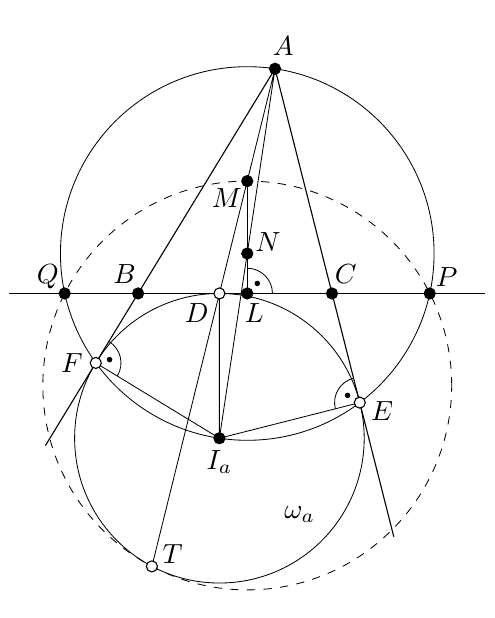
\begin{tikzpicture}[x=1.25cm,y=1.25cm]
			\coordinate (A) at (0,2.283);
			\coordinate (B) at (-1.391,0);
			\coordinate (C) at (0.579,0);
			\coordinate (D) at (-0.565,0);
			\coordinate (E) at (0.861,-1.109);
			\coordinate (F) at (-1.821,-0.706);
			\coordinate (Ia) at (-0.565,-1.471);
			\coordinate (L) at (-0.282,0);
			\coordinate (M) at (-0.282,1.141);
			\coordinate (N) at (-0.282,0.406);
			\coordinate (P) at (1.572,0);
			\coordinate (Q) at (-2.137,0);
			\coordinate (T) at (-1.251,-2.773);
			\draw[line width=0.3] (Ia) circle (1.471);
			\draw[line width=0.3] (N) circle (1.898);
			\draw[line width=0.3,dashed] (-0.282,-0.935) circle (2.077);
			\draw[shorten >=-2em,shorten <=-2em] (P) to (Q);
			\draw[shorten >=-5em] (A) to (E);
			\draw[shorten >=-3.5em] (A) to (F);
			\draw[line width=0.3] (T) to (A) to (Ia) to (D);
			\draw[line width=0.3] (M) to (L);
			\draw[line width=0.3] (E) to (Ia) to (F);
			\draw [line width=0.3,shift={(L)}] (0:0.32cm) arc (0:90:0.32cm);
			\fill [shift={(L)}] (45:0.18cm) circle (1pt);
			\draw [line width=0.3,shift={(E)}] (104.242:0.32cm) arc (104.242:194.242:0.32cm);
			\fill [shift={(E)}] (149.242:0.18cm) circle (1pt);
			\draw [line width=0.3,shift={(F)}] (328.642:0.32cm) arc (328.642:418.642:0.32cm);
			\fill [shift={(F)}] (373.642:0.18cm) circle (1pt);
			\draw[fill=black] (A) circle (2pt) node[shift={(70:2ex)}] {$A$};
			\draw[fill=black] (B) circle (2pt) node[shift={(125:2ex)}] {$B$};
			\draw[fill=black] (C) circle (2pt) node[shift={(55:2ex)}] {$C$};
			\draw[fill=white] (D) circle (2pt) node[shift={(220:2.5ex)}] {$D$};
			\draw[fill=white] (E) circle (2pt) node[shift={(-20:2ex)}] {$E$};
			\draw[fill=white] (F) circle (2pt) node[shift={(180:2ex)}] {$F$};
			\draw[fill=black] (Ia) circle (2pt) node[shift={(270:2ex)}] {$I_a$};
			\draw[fill=black] (L) circle (2pt) node[shift={(290:1.75ex)}] {$L$};
			\draw[fill=black] (M) circle (2pt) node[shift={(220:2.25ex)}] {$M$};
			\draw[fill=black] (N) circle (2pt) node[shift={(30:2ex)}] {$N$};
			\draw[fill=black] (P) circle (2pt) node[shift={(45:2ex)}] {$P$};
			\draw[fill=black] (Q) circle (2pt) node[shift={(135:2ex)}] {$Q$};
			\draw[fill=white] (T) circle (2pt) node[shift={(30:2ex)}] {$T$};
			\node at (0.25,-2.25) {$\omega_a$};
		\end{tikzpicture}
	\end{figure}
	
	Nach dem Kreisberührungslemma gilt $\abs{MD}\cdot \abs{MT}=\abs{MP'}^2$. Andererseits ist $M$ der Mittelpunkt von $\overline{AD}$, also gilt $\abs{MD}\cdot \abs{MT}=\abs{AM}\cdot \abs{MT}=\abs{AM}\cdot \abs{AT}-\abs{AM}^2=\frac12\abs{AD}\cdot\abs{AT}-\frac14\abs{AD}^2$. Nach dem Sekanten-Tangentensatz und Aufgabe~\ref{aufgabe:s-a} ist $\abs{AD}\cdot \abs{AT}=\abs{AE}^2=s^2$. Den Term $\abs{AD}^2$ können wir mit dem Satz des Pythagoras (oder mit dem Satz von Stewart) ausrechnen. Dazu bezeichne $h_a$ die Länge der Höhe von~$A$ auf $BC$. Nach Aufgabe~\ref{aufgabe:s-a} ist $\abs{CD}=s-b$ und außerdem hat die Strecke zwischen $C$ und dem Lotfußpunkt von $A$ auf $BC$ die Länge $b\cos\gamma$. Es folgt $\abs{AD}^2=h_a^2+\parens*{(s-b)-b\cos\gamma}^2$. Schließlich folgt aus dem Satz von Pythagoras die Gleichung $\abs{P'L}^2=\abs{MP'}^2-\abs{ML}^2=\abs{MP'}^2-\frac14h_a^2$. Indem wir alles einsetzen, erhalten wir
	\begin{align*}
		\abs{P'L}^2&=\frac{\abs{AD}\cdot \abs{AT}}{2}-\frac{\abs{AD}^2}{4}-\frac{h_a^2}{4}=\frac{s^2}{2}-\frac{h_a^2}{2}-\frac{\parens[\big]{(s-b)-b\cos\gamma}^2}{4}\\
		&=\frac{s^2}{2}-\frac{2\mathrm{A}^2}{a^2}-\frac{\parens*{\frac{a-b+c}{2}-b\cdot \frac{a^2+b^2-c^2}{2ab}}^2}{4}=\frac{s^2}{2}-\frac{2s(s-a)(s-b)(s-c)}{a^2}-\frac{(b-c)^2s^2}{4a^2}\\
		&=\frac{s\parens*{2a^2s-8(s-a)(s-b)(s-c)-(b-c)^2s}}{4a^2}\,.
	\end{align*}
	Hier haben wir die folgenden Formeln eingesetzt: Zuerst $h_a=2\mathrm{A}/a$ nach der üblichen Flächeninhaltsformel, dann $s-b=(a-b+c)/2$ nach Definition und $\cos\gamma=(a^2+b^2-c^2)/(2ab)$ nach dem Cosinusssatz und schließlich $\mathrm{A}=\sqrt{s(s-a)(s-b)(s-c)}$ nach dem Satz von Heron.
	
	Spätestens an diesem Punkt ist klar, dass sich die Aufgabe durchrechnen lässt, denn wir haben es geschafft, den Term $\abs{P'L}^2$, der von dem komplizierten Punkt~$T$ abhängt, nur durch die Dreiecksseiten auszudrücken. Der Term $\abs{PL}^2$ sollte einfacher sein, weil er nicht von~$T$ abhängt.
	
	Diesen Term nehmen wir uns jetzt vor. Sei~$I_a$ der Ankreismittelpunkt und~$r_a$ der Ankreisradius. Weil $AE$ und $AF$ Tangenten an den Ankreis~$\omega_a$ sind, gilt $\winkel AEI_a=90^\circ=\winkel I_aFA$. Nach Thales ist der Umkreismittelpunkt von $\odot AEF$ also der Mittelpunkt~$N$ von $\overline{AI_a}$. Folglich liegt~$N$ auf der Mittelsenkrechten von $\overline{AE}$. Wegen $\abs{AE}=s$ und $\winkel NAE=\winkel I_aAE=\alpha/2$ erhalten wir $\abs{NA}=s/(2\cos(\frac\alpha2))$. Weil $P$ auf dem Umkreis $\odot AEF$ liegt, dessen Mittelpunkt~$N$ ist, gilt $\abs{PN}=\abs{AN}$. Aus dem Strahlensatz ist klar, dass $N$ auch auf der Geraden $ML$ liegt, also folgt $\abs{PL}^2=\abs{PN}^2-\abs{NL}^2=\abs{AN}^2-\abs{NL}^2$ nach Pythagoras. Schließlich gilt nach Strahlensatz $\abs{MN}=\frac12\abs{DI_a}=\frac12r_a$, folglich $\abs{NL}=\abs{ML}-\abs{MN}=\frac12(h_a-r_a)$. Indem wir wiederum alles einsetzen, erhalten wir
	\begin{align*}
		\abs{PL}^2&=\abs{AN}^2-\abs{NL}^2=\parens*{\frac{s}{2\cos\parens[\big]{\frac\alpha2}}}^2-\frac{h_a^2}{4}-\frac{r_a^2}{4}+\frac{r_ah_a}{2}\\
		&=\frac{s^2}{4}\cdot\frac{bc}{s(s-a)}-\frac{\mathrm{A}^2}{a^2}-\frac{\mathrm{A}^2}{4(s-a)^2}+\frac{\mathrm{A}^2}{a(s-a)}\\
		&=\frac{s\parens*{a^2bc-4(s-a)^2(s-b)(s-c)-a^2(s-b)(s-c)+4a(s-a)(s-b)(s-c)}}{4a^2(s-a)}
	\end{align*}
	Hier haben wir nacheinander die Halbwinkelformel $\cos(\frac\alpha2)=(s(s-a))/(bc)$, die Flächeninhaltsformel $h_a=2\mathrm{A}/a$, die Formel $r_a=\mathrm{A}/(s-a)$ sowie den Satz von Heron eingesetzt. Im letzten Schritt haben wir außerdem schon einmal $s-a$ gekürzt. Wegen $a^2bc-a^2(s-b)(s-c)=a^2s(s-a)$ lässt sich der Faktor~$s-a$ ein weiteres mal kürzen und wir erhalten
	\begin{equation*}
		\abs{PL}^2=\frac{s\parens*{a^2s-4(s-a)(s-b)(s-c)+4a(s-b)(s-c)}}{4a^2(s-a)}
	\end{equation*}
	Indem wir diesen Term mit dem Term für $\abs{P'L}^2$ vergleichen, sehen wir, dass wir nur noch $a^2s-(b-c)^2s=4(s-a)(s-b)(s-c)+4a(s-b)(s-c)$ zeigen müssen. Das ist nun klar, denn beide Terme lassen sich unmittelbar zu $4s(s-b)(s-c)$ umformen.
\end{proof}

\subsection*{Komplex durchrechnen}
\textbf{Grundbegriffe.} Die Menge der \emph{komplexen Zahlen} $\mathbb C$ entsteht, indem wir zu den reellen Zahlen $\mathbb R$ eine \emph{imaginäre Einheit} $\mathrm{i}$ hinzufügen, die $\mathrm{i}^2=-1$ erfüllt. Eine allgemeine komplexe Zahl ist dann durch $z=x+\mathrm{i}y$ gegeben, wobei $x$ und $y$ reelle Zahlen sind.

Die komplexen Zahlen haben eine Reihe von Vorteilen gegenüber den reellen Zahlen. Zum Beispiel ist sofort klar, dass sich alle quadratischen Gleichungen in $\mathbb C$ lösen lassen, denn das Hinzufügen von $\mathrm{i}$ erlaubt uns, auch Wurzeln aus negativen Zahlen zu ziehen. Tatsächlich gilt das nicht nur für quadratische Gleichungen: In $\mathbb C$ lassen sich \emph{alle} polynomiellen Gleichungen lösen, egal von welchem Grad!\footnote{Diesen Fakt haben wir bereits in Kapitel~\ref{kapitel:Rekursionen}: \emph{Lineare Rekursionen} verwendet.} Dieser Fakt wird auch als \emph{Fundamentalsatz der Algebra} bezeichnet. Einen Beweis für die werdet ihr im Studium sehen; er würde hier zu weit führen.

Wir wollen in diesem Kapitel erklären, wie sich komplexe Zahlen in der Geometrie verwenden lassen. Die Grundidee ist folgende: Statt Punkte in der Ebene durch Koordinaten $(x,y)$ zu beschreiben, können wir sie auch als komplexe Zahlen $z=x+\mathrm{i} y$ auffassen. Die reellen Zahlen liegen dann auf der $x$-Achse, während die \emph{rein imaginären} Zahlen, also die komplexen Zahlen der Form $0+\mathrm{i} y$, auf der $y$-Achse liegen. Deshalb werden wir im Folgenden stattdessen von der \emph{reellen} und der \emph{imaginären Achse} sprechen.
	
\begin{wrapfigure}{r}{0.25\textwidth}
	\centering\vspace{-0.44cm}
	\begin{tikzpicture}
		\draw[->] (-0.5,0) to node[pos=1,below=0.5ex] {$\mathbb R$} (3,0);
		\draw[->] (0,-1.6) to node[below left] {$0$} node[pos=1,right=0.5ex] {$\mathrm{i}\mathbb R$} (0,1.6);
		\coordinate (z) at (24:2.2);
		\coordinate (zbar) at (-24:2.2);
		\draw [line width=0.3] (0,0) to node[shift={(114:1.5ex)}] {$r$} (z);
		\draw [line width=0.3,dashed] (z) to (zbar);
		\draw (z) node [above right] {$z$} ++(-0.5ex,-0.5ex) to ++(1ex,1ex) ++(0ex,-1ex) to ++(-1ex,1ex);
		\draw (zbar) node [below right] {$\overline z$} ++(-0.5ex,-0.5ex) to ++(1ex,1ex) ++(0ex,-1ex) to ++(-1ex,1ex);
		\draw [line width=0.3] (0:1.25cm) arc (0:24:1.25cm);
		\node at (12:1cm) {$\varphi$};
	\end{tikzpicture}
	Betrag, Argument und Konjugiertes\vspace{-0.5cm}
\end{wrapfigure}
Der \emph{Betrag von~$z$} ist definiert als $\abs{z}\coloneqq \sqrt{x^2+y^2}$, also als der Abstand zum Ursprung. Wenn $r=\abs{z}$, dann können wir $z$ auch in \enquote{Polarkoordinaten} als $z=r(\cos\varphi+\mathrm{i}\sin\varphi)$ schreiben, wobei $\varphi$ der Winkel ist, den die Strecke von $0$ nach~$z$ mit der reellen Achse einschließt. Wir nennen $\varphi$ auch das \emph{Argument von~$z$}. Die komplexe Zahl $x-\mathrm{i} y$, also das Spiegelbild von~$z$ an der reellen Achse, nennen wir die \emph{zu~$z$ konjugierte komplexe Zahl}, und wir schreiben $\overline{z}\coloneqq x-\mathrm{i} y$.

\textbf{Rechnen mit komplexen Zahlen.} Wir können komplexe Zahlen wie gewohnt addieren, subtrahieren und multiplizieren. Nach der dritten binomischen Formel gilt dann 
\begin{equation*}
	z\overline{z}=(x+\mathrm{i} y)(x-\mathrm{i} y)=x^2-\mathrm{i}^2y^2=x^2+y^2=\abs{z}^2\,.
\end{equation*}
Diese Beobachtung erlaubt uns, auch durch komplexe Zahlen zu dividieren (außer durch~$0$ natürlich), denn wir können 
\begin{equation*}
	\frac{z_1}{z_2}=\frac{1}{\abs{z_2}^2}\cdot z_1\overline{z_2}
\end{equation*}
schreiben (und $1/\abs{z_2}^2$ ist schon definiert, denn $\abs{z_2}$ ist ja eine reelle Zahl). Ihr könnt euch leicht überlegen, dass sich die komplexe Konjugation mit Addition, Subtraktion, Multiplikation und Division verträgt,
% Tien: Kommutieren ist das falsche Wort. Viel eher verhält es sich distributiv über den Grundrechenarten.
das heißt es es gilt
\begin{equation*}
	\overline{z_1+z_2}=\overline{z_1}+\overline{z_2},\quad
	\overline{z_1-z_2}=\overline{z_1}-\overline{z_2},\quad
	\overline{z_1\cdot z_2}=\overline{z_1}\cdot \overline{z_2}\quad
	\text{und}\quad
	\overline{z_1/z_2}=\overline{z_1}/\overline{z_2}\,.
\end{equation*}

\textbf{Multiplikation als Drehstreckung.}
Bei der Multiplikation von komplexen Zahlen in Polarkoordinaten ergibt sich nun etwas Interessantes: Wenn nämlich $z_1=r_1(\cos\varphi_1+\mathrm{i}\sin\varphi_1)$ und $z_2=r_2(\cos\varphi_2+\mathrm{i}\sin\varphi_2)$ ist, dann gilt
\begin{align*}
	z_1z_2&=r_1r_2\parens[\Big]{\parens[\big]{\cos\varphi_1\cos\varphi_2-\sin\varphi_1\sin\varphi_2}+\mathrm{i}\parens[\big]{\sin\varphi_1\cos\varphi_2+\cos\varphi_1\sin\varphi_2}}\\
	&=r_1r_2\parens[\big]{\cos(\varphi_1+\varphi_2)+\mathrm{i}\sin(\varphi_1+\varphi_2)}\,,
\end{align*}
worin wir die Additionstheoreme für Sinus und Cosinus erkannt haben. Wenn wir also mit einer komplexen Zahl $z=r(\cos\varphi+\mathrm{i}\sin\varphi)$ multiplizieren, dann multiplizieren wir den Betrag mit~$r$ und addieren~$\varphi$ zum Argument. Mit anderen Worten: \emph{Multiplikation mit~$z$ ist eine Drehstreckung um den Punkt~\(0\), mit Streckfaktor~$r$ und Drehwinkel~$\varphi$!}

\textbf{Geometrie mit komplexen Zahlen.}
Mithilfe dieser Beobachtung können wir effektiv Geometrie mit komplexen Zahlen betreiben. Betrachte zum Beispiel vier Punkte $A$,~$B$, $C$ und~$D$ in der Ebene. Seien $a$,~$b$, $c$ und~$d$ die entsprechenden komplexen Zahlen. Dann stehen die Geraden $AB$ und~$CD$ genau dann senkrecht aufeinander, wenn die Drehstreckung, die durch Multiplikation mit der komplexen Zahl $z\coloneqq (a-b)/(c-d)$ gegeben ist, den Winkel $90^\circ$ oder~$270^\circ$ hat. Also gilt $AB\perp CD$ genau dann, wenn das Argument von~$z$ durch $90^\circ$ oder~$270^\circ$ gegeben ist. Das wiederum ist äquivalent dazu, dass $z$ rein imaginär ist, was wir mithilfe der komplexen Konjugation ein weiteres Mal zu $z=-\overline{z}$ äquivalent umformen können. Wir erhalten also, dass $AB$ und $CD$ genau dann senkrecht aufeinander stehen, wenn
\begin{equation*}
	\frac{a-b}{c-d}=-\frac{\overline{a}-\overline{b}}{\overline{c}-\overline{d}}
\end{equation*}
gilt. Eine ähnliche Überlegung verrät uns, dass $AB$ und~$CD$ genau dann parallel sind, wenn $z\coloneqq (a-b)/(c-d)$ das Argument $0^\circ$ oder~$180^\circ$ hat. Das ist wiederum äquivalent dazu, dass $z$ reell ist, was wir auch durch die Bedingung $z=\overline{z}$ ausdrücken können. Also sind $AB$ und~$CD$ genau dann parallel, wenn
\begin{equation*}
	\frac{a-b}{c-d}=\frac{\overline{a}-\overline{b}}{\overline{c}-\overline{d}}\,.
\end{equation*}
Ein Punkt~$X$ liegt auf der Geraden~$AB$ genau dann, wenn $AX$ und~$AB$ parallel sind. Mit den obigen Überlegungen ist das äquivalent zu der Gleichung
\begin{equation*}
	\frac{x-a}{b-a}=\frac{\overline{x}-\overline{a}}{\overline{b}-\overline{a}}\,.
\end{equation*}
Wir können also Geraden in komplexen Zahlen beschreiben.

Ähnlich verhält es sich mit Kreisen. Seien $A$,~$B$, $C$ und~$X$ vier Punkte in der Ebene und seien $a$,~$b$, $c$ und~$x$ die zugehörigen komplexen Zahlen. Wir nehmen der Einfachheit halber an, dass $C$~und~$X$ in der gleichen Halbebene bezüglich~$AB$ liegen. Nach dem Peripheriewinkelsatz liegt $X$ genau dann auf dem Umkreis $\odot ABC$, wenn $\winkel AXB=\winkel ACB$. Das ist genau dann der Fall, wenn die Drehstreckungen, die durch Multiplikation mit den komplexen Zahlen $z_1\coloneqq (a-x)/(b-x)$ und $z_2\coloneqq (a-c)/(b-c)$ gegeben sind, den gleichen Drehwinkel haben. Die komplexen Zahlen $z_1$~und~$z_2$ müssen also das gleiche Argument haben. Das wiederum ist äquivalent dazu, dass $z_1/z_2$ das Argument~$0^\circ$ hat, also eine nichtnegative reelle Zahl ist. Wenn $X$~und~$C$ in verschiedenen Halbebenen bezüglich~$AB$ liegen, erhalten wir analog die Bedingung, dass $z_1/z_2$ das Argument~$180^\circ$ hat, also eine nichtpositive reelle Zahl ist. Insgesamt sehen wir, dass $X$ genau dann auf dem Umkreis $\odot ABC$ liegt, wenn $z_1/z_2$ reell ist, also genau dann, wenn
\begin{equation*}
	\frac{a-x}{b-x}\bigg/\frac{a-c}{b-c}=\frac{\overline{a}-\overline{x}}{\overline{b}-\overline{x}}\bigg/\frac{\overline{a}-\overline{c}}{\overline{b}-\overline{c}}\,.
\end{equation*}

\begin{aufgabe*}
	Betrachte sechs Punkte $A$,~$B$,~$C$ und $A'$,~$B'$,~$C'$. Seien $a$,~$b$,~$c$ und $a'$,~$b'$,~$c'$ die entsprechenden komplexen Zahlen. Zeige, dass die Dreiecke $ABC$ und $A'B'C'$ genau dann gleichsinnig ähnlich sind, wenn folgendes gilt:
	\begin{equation*}
		\frac{b-a}{c-a}=\frac{b'-a'}{c'-a'}\,.
	\end{equation*}
\end{aufgabe*}

Wir werden nun an einem Beispiel demonstrieren, wie sich Olympiadeaufgabe mit komplexen Zahlen durchrechnen lassen.

\begin{aufgabe*}
	Gegeben sei ein konvexes Fünfeck $ABCDE$ mit $\winkel CBA=\winkel AED=90^\circ$. Der Mittelpunkt des Umkreises $\odot ABE$ sei~$M$ und der Mittelpunkt des Umkreises $\odot ACD$ sei~$O$. Beweise: Wenn $M$ der Mittelpunkt der Strecke~$\overline{CD}$ ist, dann verläuft die Gerade~$AO$ durch den Mittelpunkt der Strecke~$\overline{BE}$.
\end{aufgabe*}

\begin{proof}[Lösung]
	Wir beginnen zuerst mit einigen elementaren Beobachtungen (was, wie bereits erwähnt, immer eine gute Idee ist). Sei $X$ der Schnittpunkt der Geraden $BC$ und~$DE$ (diese können nicht parallel sein, sonst würde das Fünfeck bei~$A$ entarten). Wegen $\winkel XBA=\winkel AEX=90^\circ$ ist $\overline{AX}$ ein Durchmesser des Umkreises $\odot ABE$. Der Umkreismittelpunkt~$M$ muss also auch der Mittelpunkt von~$\overline{AX}$ sein. Das Viereck $ACXD$ muss also ein Parallelogramm sein, denn seine Diagonalen halbieren sich.
	
	
	% Tien: Im Bild fehlen z.B. O und BE, aber wenn es nicht passt, ist es auch okay.
	\begin{figure}[ht]
		\centering
		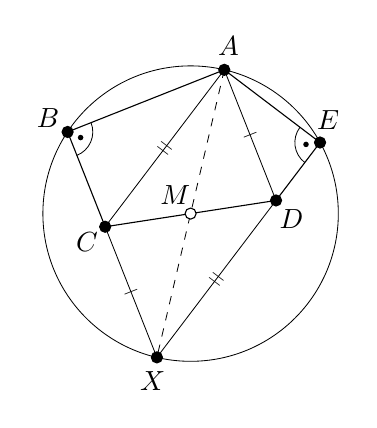
\begin{tikzpicture}
			\coordinate (M) at (-0.144,0.464);
			\coordinate (A) at (0.284,2.29);
			\coordinate (B) at (-1.706,1.501);
			\coordinate (C) at (-1.229,0.297);
			\coordinate (D) at (0.941,0.631);
			\coordinate (E) at (1.5,1.367);
			\coordinate (X) at (-0.572,-1.362);
			\draw [line width=0.3] (M) circle (1.876);
			\draw (A) to (B) to (C) to (D) to (E) to cycle;
			\draw [line width=0.3] (C) to node[sloped] {$\scriptscriptstyle|$} (X) to node[sloped] {$\scriptscriptstyle||$} (D) to node[sloped] {$\scriptscriptstyle|$} (A) to node[sloped] {$\scriptscriptstyle||$} cycle;
			\draw [line width=0.3,dashed] (A) to (X);
			\draw [line width=0.3, shift={(B)}] (-68.385:0.32cm) arc (-68.385:21.615:0.32cm);
			\fill [shift={(B)}] (-23.315:0.18cm) circle (1pt);
			\draw [line width=0.3, shift={(E)}] (142.795:0.32cm) arc (142.795:232.795:0.32cm);
			\fill [shift={(E)}] (187.795:0.18cm) circle (1pt);
			\draw[fill=white] (M) circle (2pt) node[shift={(130:2ex)}] {$M$};
			\draw[fill=black] (A) circle (2pt) node[shift={(80:2ex)}] {$A$};
			\draw[fill=black] (B) circle (2pt) node[shift={(145:2ex)}] {$B$};
			\draw[fill=black] (C) circle (2pt) node[shift={(220:2ex)}] {$C$};
			\draw[fill=black] (D) circle (2pt) node[shift={(-50:2ex)}] {$D$};
			\draw[fill=black] (E) circle (2pt) node[shift={(70:2ex)}] {$E$};
			\draw[fill=black] (X) circle (2pt) node[shift={(260:2ex)}] {$X$};
		\end{tikzpicture}
	\end{figure}
	
	Nun rechnen wir komplex durch. Die zu $A$,~$B$,~\ldots\ gehörigen komplexen Zahlen bezeichnen wir mit $a$,~$b$,~\dots\
	% Tien: Soweit ich weiß, werden im Deutschen nach Ellipsen kein Satzschlusspunkt gesetzt.
	Ohne Einschränkung dürfen wir annehmen, dass $\odot ACD$ der komplexe Einheitskreis ist (es ist immer praktisch, einen geeigneten Kreis auf den Einheitskreis zu legen). Dann gilt $1=\abs{a}^2=a\overline{a}$, also $\overline{a}=1/a$. Analog folgt $\overline{c}=1/c$ und $\overline{d}=1/d$. Der Mittelpunkt des komplexen Einheitskreises ist~$0$, also gilt $O=0$.
	
	Weil $B$~auf~$CX$ liegt und $ACXD$ ein Parallelogramm ist, müssen $BC$ und~$AD$ parallel sein. Wir erhalten also
	\begin{equation*}%\label{eq:Komplex1}
		\frac{b-c}{d-a}=\frac{\overline{b}-\overline{c}}{\overline{d}-\overline{a}}\quad\Longleftrightarrow\quad \overline{b}-\overline{c}=(b-c)\parens*{\frac{\overline{d}-\overline{a}}{d-a}}=-\frac{b-c}{ad}\,.
	\end{equation*}
	Im letzten Schritt haben wir $\overline{a}=1/a$ und $\overline{d}=1/d$ eingesetzt, um $(\overline{d}-\overline{a})/(d-a)=-1/(ad)$ zu erhalten. (Vereinfachungen von dieser Sorte sind einer der Gründe, warum es praktisch ist, möglichst viele Punkte auf den Einheitskreis zu legen\@.) Nach Voraussetzung ist ferner $AB\perp BC$. Wegen $AD\parallel BC$ muss auch $AB\perp AD$ sein. Wir erhalten also
	\begin{equation*}%\label{eq:Komplex2}
		\frac{a-b}{d-a}=-\frac{\overline{a}-\overline{b}}{\overline{d}-\overline{a}}\quad\Longleftrightarrow \quad \overline{b}-\overline{a}=(a-b)\parens*{\frac{\overline{d}-\overline{a}}{d-a}}=-\frac{a-b}{ad}\,,
	\end{equation*}
	wobei wir wieder $\overline{a}=1/a$ und $\overline{d}=1/d$ eingesetzt haben. Indem wir die Gleichungen für $\overline{b}-\overline{a}$ und $\overline{b}-\overline{c}$ voneinander subtrahieren, erhalten wir
	\begin{equation*}%\label{eq:Komplex3}
		\overline{c}-\overline{a}=\frac{2b-(a+c)}{ad}\quad\Longleftrightarrow\quad b=\frac{a+c+ad(\overline{c}-\overline{a})}{2}=\frac{ac+c^2+ad-cd}{2c}\,,
	\end{equation*}
	wobei wir im letzten Schritt $\overline{a}=1/a$ und $\overline{c}=1/c$ eingesetzt haben. Aus Symmetriegründen lässt sich $e$ völlig analog berechnen; dabei werden lediglich die Rollen von $c$~und~$d$ vertauscht. Wir erhalten also
	\begin{equation*}%\label{eq:Komplex4}
		e=\frac{ad+d^2+ac-cd}{2d}\,.
	\end{equation*}
	Der Mittelpunkt von $\overline{BE}$ entspricht offensichtlich der komplexen Zahl $(b+e)/2$. Aus den Gleichungen für~$b$ und~$e$ folgt
	\begin{equation*}%\label{eq:Komplex5}
		\frac{b+e}{2}=\frac{(ac+c^2+ad-cd)d+(ad+d^2+ac-cd)c}{4cd}=\frac{2acd+ad^2+ac^2}{4cd}=a\frac{(c+d)^2}{4cd}\,.
	\end{equation*}
	Um zu zeigen, dass $A$,~$O$ und der Mittelpunkt von~$\overline{BE}$ kollinear sind, können wir die allgemeine Bedingung verwenden und werden zweifellos nach kurzer Rechnung zum Ziel kommen. Wir können uns aber noch ein wenig schlauer anstellen: Wegen $O=0$ müssen wir lediglich zeigen, dass $(b+e)/2$ ein reelles Vielfaches von~$a$ ist. Dank der Gleichung für $(b+e)/2$ müssen wir also nur zeigen, dass der Faktor $(c+d)^2\!/(4cd)$ eine reelle Zahl ist. Wegen $\overline{c}=1/c$ und $\overline{d}=1/d$ erhalten wir $\overline{c}+\overline{d}=(c+d)/(cd)$, also ist $(c+d)^2\!/(4cd)=\frac14(c+d)(\overline{c}+\overline{d})=\frac 14\abs{c+d}^2$. Dieser Ausdruck ist definitiv eine reelle Zahl und wir sind fertig.
\end{proof}